\documentclass[runningheads,a4paper]{llncs}
\usepackage[utf8x]{inputenc}
\usepackage[pdftex]{graphicx}
%\usepackage{graphicx}
\usepackage{amssymb}
\usepackage{url}
\usepackage{a4wide}
\setcounter{tocdepth}{3}
\usepackage[spanish]{babel}

\urldef{\mails}\path|{cgcossio,mailen.gomezmayol, miguelmsoler}@gmail.com|
\newcommand{\keywords}[1]{\par\addvspace\baselineskip
\noindent\keywordname\enspace\ignorespaces#1}

\begin{document}
\mainmatter

\title{Detección de Rasgos en la Identificación de Letras Utilizando Bubbles}
\titlerunning{Detección de Rasgos Utilizando Bubbles}
\author{Christian Cossio Mercado \and Mail\'en G\'omez Mayol \and Miguel Mart\'inez Soler}
\authorrunning{Detección de Rasgos Utilizando Bubbles}

\institute{Facultad de Ciencias Exactas y Naturales, UBA\\Buenos Aires, Argentina\\\mails }
\toctitle{Detección de Rasgos Utilizando Bubbles}
\tocauthor{Cossio Mercado, Gomez Mayol, Martinez Soler}

\maketitle
\begin{abstract}
El reconocimiento de letras\ldots
\keywords{Identificaci\'on de Letras, Detecci\'on de rasgos, Bubbles}
\end{abstract}

% + Revisión bibliográfica, 
% + experimento viejo
% + variación propuesta. 
% + Diseño experimentaldetallado 

\section{Introducción}
\label{sec:Introduccion}
\ldots

\subsection{Objetivo}
Reconocer rasgos utilizados por una persona para reconocer letras, presentadas utilizando diferentes tipografías.

\subsection{Revisi\'on Bibliográfica}
\label{sec:RevisionBibliografica}
\ldots


\section{Hipótesis}

A partir de la definición particular del experimento de este trabajo, así como por lo registrado en trabajos anteriores relacionados con el reconocimiento de letras, se definió el siguiente conjunto de hipótesis a verificar:
\begin{enumerate}
 \item El conjunto de rasgos detectados no es idiosincrático al grupo de individuos participantes en el experimento (i.e., se trata de una forma de identificación del ser humano en general).
    \subitem Hipótesis nula (H0): El conjunto de rasgos detectados es propio de cada grupo de individuos analizado. 
    \subitem Refutación (Ref): Fuera del alcance de este experimento. Sólo se realizará el análisis de comparación de los rasgos obtenidos en \cite{FisetEtAl08:BubblesForLetters}.
 \item El uso de tipografías ampliamente conocidas (por ej., la de Coca-Cola) facilita el reconocimiento de las letras.
    \subitem Hipótesis nula (H0): El uso de tipografías conocidas no mejora la performance en comparación con otras letras de la misma complejidad.
    \subitem Refutación (Ref): En comparación con las otras dos tipografías, la tasa de aciertos de una letra debería comportarse linealmente con respecto a su complejidad.
 \item Aún en casos en los que el sujeto no cree haber visto --- o ni siquiera conoce --- alguna tipografía famosa, el porcentaje de aciertos mejora significativamente.
    \subitem H0: No hay variaciones en la performance para letras vistas durante el experimento, ni para aquellas definidas como conocidas.
    \subitem Ref:
 \item A mayor complejidad de las letras, menor eficiencia en el reconocimiento \cite{PelliEtAl06:LetterIdentification}
    \subitem H0: 
    \subitem Ref:
 \item Los rasgos de una letra (e.g., 'b') varían de acuerdo a la tipografía que se esté utilizando \cite{PelliEtAl06:LetterIdentification}.
    \subitem H0: 
    \subitem Ref:
 \item Habrá una variación en los rasgos de la letra `n' con relación a la incorporación de la letra `ñ' en todas las tipografías (cf. \cite{FisetEtAl08:BubblesForLetters}).
    \subitem H0: 
    \subitem Ref:
 \item Un observador ideal utilizará rasgos distintos a los que utiliza un ser humano para la identificación de las letras \cite{PelliEtAl06:LetterIdentification}.
    \subitem H0: 
    \subitem Ref:
\end{enumerate}



\section{Dise\~no del Experimento}
\label{sec:DisenoExperimento}

\subsection{Participantes}

Del experimento participaron 6 personas, de entre 20 y 33 años, con visión normal o corregida.

\subsection{Est\'imulos presentados'}
Letras del alfabeto español, en mayúscula y minúscula (incluyendo ñ).
Tres tipografías: Arial, Kunstler y otra de letras reconocidas (denominadas Famosas).

Se generó 16 bloques de 100 estímulos cada una, donde se presentó mitad de los estímulos en mayúsculas y luego la otra mitad en minúscula.

A cada estímulo se le aplicó un filtrados por bandas de frecuencia, de manera de mostrar información de 32 a 16 ciclos/letra,

\begin{figure}
 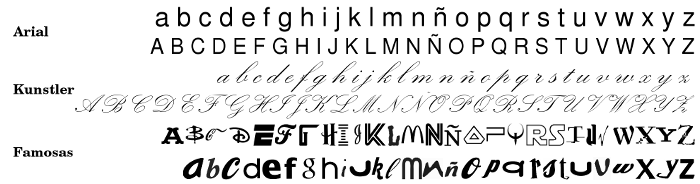
\includegraphics[scale=0.23]{letras.png}
  \caption{Conjunto completo de letras utilizadas en el experimento}
  \label{figura:conjuntoLetras}
\end{figure}


\subsection{Procedimiento}


\section{Resultados}
\ldots

\subsection{Mediciones realizadas}
\ldots
\begin{itemize}
 \item Porcentaje de aciertos promedio por estímulo
 \item Porcentaje de aciertos y tiempo promedio de respuesta en función de la complejidad
 \item 

\end{itemize}


\section{Discusi\'on}
\ldots

\section{Conclusiones}
\ldots


\newpage

\begin{thebibliography}{20}
  \bibitem{AttneaveArnoult:QuantitativeStudyOfShape}	Attneave, F. \& Arnoult, M.: The quantitative study of shape and pattern perception (1956)
  \bibitem{Chauvin05:TestsForClassificationImages}	Chauvin, A., Worsley, K.J., Schyns, P., Arguin, M. \& Gosselin, F.: Accurate statistical tests for smooth classification images (2005)
  \bibitem{FarellPelli99:MeasureThreshold}		Farell, B. \& Pelli, D.: Psychophysical methods, or how to measure a threshold and why (1999)
  \bibitem{FisetEtAl08:BubblesForLetters}		Fiset, D. \& Blais, C., \'Ethier-Majcher, C., Arguin, M., Bub, D., Gosselin, F.: Features for Identification of Uppercase and Lowercase Letters (2008)
  \bibitem{FisetEtAl09:SpatioTemporalBubbles}		Fiset, D. et al: The spatio-temporal dynamics of visual letter recognition (2009)
  \bibitem{GosselinSchyns01:Bubbles}			Gosselin, F. \& Schyns, P.: Bubbles. a technique to reveal the use of information in recognition tasks (2001)
  \bibitem{GosselinSchyns03:BubblesUsersGuide}		Gosselin, F. \& Schyns, P.: A User's Guide to Bubbles (2003)
  \bibitem{GraingeEtAl08:LetterPerception}		Grainger et al: Letter Perception. from pixels to pandemonium (2008)
  \bibitem{OrucLandy09:ChannelSwitching}		Oruc, I. \& Landy, M.: Scale dependence and channel switching in letter identification (2009)
  \bibitem{PelliFarell10:PychophysicalMethods}		Pelli, D. \& Farell, B.: Psychophysical Methods (2010)
  \bibitem{Pelli01:HowWeSeeLetters}			Pelli, D.: How We See Letters. Implications for Making Better Displays (2001)
  \bibitem{Pelli03:InnefOfWordRecognition}		Pelli, D.: The remarkable inefficiency of word recognition (2003)
  \bibitem{PelliEtAl09:GestaltInLetterIdentif}		Pelli, D. et al: Grouping in Object Recognition. The role of a Gestalt law in letter identification (2009)
  \bibitem{PelliEtAl06:LetterIdentification}		Pelli, D., Burns, C.W., Farell, B. \& Moore-Page, D.C.: Feature detection and letter identification (2006)
  \bibitem{PetitGrainger02:PrimingForLetterPercept}	Petit, J.P. \& Grainger. J.: Masked partial priming of letter perpection (2002)
  \bibitem{PetitEtAl06:MaskedPrimingERP}		Petit, J.P. et al: On the time course of letter perception. A masked priming ERP investigation (2006)
  \bibitem{SolomonPelli94:VisualFilterForLetterIdent}	Solomon, J. \& Pelli, D.: The Visual Filter Mediating Letter Identification (1994)


\end{thebibliography}

\end{document}
